\documentclass[12pt]{article}
\usepackage[utf8]{inputenc}
\usepackage[a4paper,top=2.5cm,bottom=2.5cm,left=2cm,right=2cm]{geometry}
\usepackage{amsmath}
%\usepackage{upgreek}
\usepackage{enumerate}
\usepackage{indentfirst}
\usepackage{subcaption}
\usepackage{graphicx}
\usepackage{caption}
\usepackage{siunitx}
\usepackage{array}
\usepackage{multirow}
\usepackage{xr}
\externaldocument[ESI-]{testfile2}

\setlength{\parindent}{4ex}

\title{Test File 1}
\author{author's name}
\date{}

\begin{document}
\maketitle

Let's include a figure.

\begin{figure}[!h]
\centering
  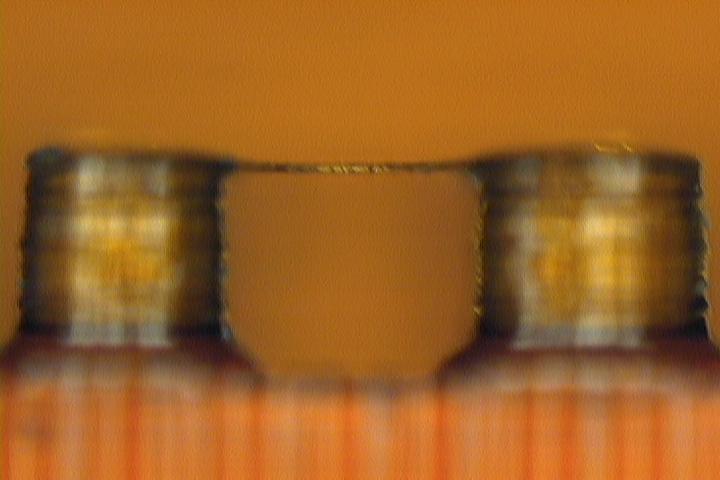
\includegraphics[width=0.5\textwidth]{10um_memb.png}
  \caption{Measured $h_a$ and $T_c$ of different resins. }
  \label{fig:10um_memb}
\end{figure}

And now we'll reference it as Fig. \ref{fig:10um_memb}.

See answer to this question for how to reference a figure in another file: http://tex.stackexchange.com/questions/14364/cross-referencing-between-different-files. Now we will reference the figure in the other file:

Fig. S\ref{ESI-fig:ha_Tc}, ESI$^\dag$.

\end{document}